\documentclass[a4paper,12pt]{article}
\usepackage{graphicx}
\usepackage{epstopdf}
\usepackage{gensymb}
%% Definitioner för LIPS-dokument

\usepackage[swedish]{babel}
\usepackage[utf8]{inputenc}
\usepackage[T1]{fontenc}
\usepackage{times}
\usepackage{ifthen}

\usepackage[margin=25mm]{geometry}

\usepackage{fancyhdr}
\pagestyle{fancy}
\lhead{}
\chead{\textbf{\LIPSprojekttitel}}
\rhead{\textbf{\textsl{LiTH}}\\\textbf{\LIPSdatum}}
\lfoot{\textbf{\LIPSkursnamn}\\\textbf{\LIPSdokumentansvarig}}
\cfoot{\textbf{\LIPSprojektgrupp}\\\textbf{\LIPSgruppepost}}
\rfoot{\textbf{\textsc{Lip}s}\\\textbf{Sida~\thepage}}

\setlength{\parindent}{0pt}
\setlength{\parskip}{1ex plus 0.5ex minus 0.2ex}


\newcommand{\twodigit}[1]{\ifthenelse{#1<10}{0}{}{#1}}
\newcommand{\dagensdatum}{\number\year-\twodigit{\number\month}-\twodigit{\number\day}}

%% ------------------------------------------
% NYBILD
% Skapar centrerad bild med caption
%   
% #1: Filens url relativt '/bilder/'
% #2:  Caption
% #3: Label
% #4: Skalning
%% ------------------------------------------
\newcommand{\nyBild}[4] 
{\begin{figure}[H]
  \centering
 \includegraphics[angle=0,scale=#4]{bilder/#1}
  \caption{#2}
  \label{fig:#3}
\end{figure}}



%%  Redefinitions of commands containing @
\makeatletter
\makeatother

\newcommand{\LIPStitelsida}{%
{\ }\vspace{45mm}
\begin{center}
  \textbf{\Huge \LIPSdokumenttyp}
\end{center}
\begin{center}
  {\Large Redaktör: \LIPSredaktor}
\end{center}
\begin{center}
  {\Large \textbf{Version \LIPSversion}}
\end{center}
\vfill
\begin{center}
  {\large Status}\\[1.5ex]
  \begin{tabular}{|*{3}{p{40mm}|}}
    \hline
    Granskad & \LIPSgranskare & \LIPSgranskatdatum \\
    \hline
    Godkänd & \LIPSgodkannare & \LIPSgodkantdatum \\
    \hline
  \end{tabular}
\end{center}
\newpage
}


\newenvironment{LIPSprojektidentitet}{%
{\ }\vspace{45mm}
\begin{center}
  {\Large PROJEKTIDENTITET}\\[0.5ex]
  {\small
  \LIPSartaltermin, \LIPSprojektgrupp\\
  Linköpings Tekniska Högskola, ISY
  }
\end{center}
\begin{center}
  {\small Gruppdeltagare}\\
%  \begin{tabular}{|p{30mm}|p{40mm}|p{35mm}|p{45mm}|}
  \begin{tabular}{|l|p{45mm}|p{25mm}|l|}
    \hline
    \textbf{Namn} & \textbf{Ansvar} & \textbf{Telefon} & \textbf{E-post} \\
    \hline
}%
{%
    \hline
  \end{tabular}
\end{center}
\begin{center}
  {\small
    \textbf{E-postlista för hela gruppen}: \LIPSgruppepost\\
    \textbf{Hemsida}: \LIPSgrupphemsida\\[1ex]
    \textbf{Kund}: \LIPSkund\\
    \textbf{Kontaktperson hos kund}: \LIPSkundkontakt\\
    \textbf{Kursansvarig}: \LIPSkursansvarig\\
    \textbf{Handledare}: \LIPShandledare\\
  }
\end{center}
\newpage
}
\newcommand{\LIPSgruppmedlem}[4]{\hline {#1} & {#2} & {#3} & {#4} \\}



\newenvironment{LIPSdokumenthistorik}{%
\begin{center}
  Dokumenthistorik\\[1ex]
  \begin{small}
    \begin{tabular}{|l|l|p{60mm}|l|l|}
      \hline
      \textbf{Version} & \textbf{Datum} & \textbf{Utförda förändringar} & \textbf{Utförda av} & \textbf{Granskad} \\
      }%
    {%
      \hline
    \end{tabular}
  \end{small}
\end{center}
}
\newcommand{\LIPSversionsinfo}[5]{\hline {#1} & {#2} & {#3} & {#4} & {#5} \\}

\newcounter{LIPSkravnummer}
\newcounter{LIPSunderkravnummer}[LIPSkravnummer]
\newenvironment{LIPSkravlista}{%
  \begin{tabular}{|p{25mm}|p{25mm}|p{85mm}|p{5mm}|}
    }%
  {%
    \hline
  \end{tabular}
}
\newcommand{\LIPSkrav}[3]{\hline\stepcounter{LIPSkravnummer}\textbf{Krav nr \arabic{LIPSkravnummer}} & \textbf{{#1}} & {#2} & \textbf{{#3}} \\}
\newcommand{\LIPSunderkrav}[3]{\hline\stepcounter{LIPSunderkravnummer}\textbf{Krav nr \arabic{LIPSkravnummer}\Alph{LIPSunderkravnummer}} & \textbf{{#1}} & {#2} & \textbf{{#3}} \\}





%%% Local Variables: 
%%% mode: latex
%%% TeX-master: "kravspec_mall"
%%% End: 



\newcommand{\LIPSartaltermin}{2012/VT}
\newcommand{\LIPSkursnamn}{TSEA27}

\newcommand{\LIPSprojekttitel}{Komborobot}

\newcommand{\LIPSprojektgrupp}{Grupp 17}
\newcommand{\LIPSgruppepost}{komborobot@googlegroups.com}
\newcommand{\LIPSgrupphemsida}{finns ej}
\newcommand{\LIPSdokumentansvarig}{Mattias Jansson}

\newcommand{\LIPSkund}{ISY, Linköpings universitet, 581\,83 Linköping}
\newcommand{\LIPSkundkontakt}{Tomas Svensson, 013-281368, tomass@isy.liu.se}
\newcommand{\LIPSkursansvarig}{Tomas Svensson, 013-281368, tomass@isy.liu.se}
\newcommand{\LIPShandledare}{}


\newcommand{\LIPSdokumenttyp}{Projektplan}
\newcommand{\LIPSredaktor}{Simon Larsson}
\newcommand{\LIPSversion}{0.1}
\newcommand{\LIPSdatum}{\dagensdatum}

\newcommand{\LIPSgranskare}{}
\newcommand{\LIPSgranskatdatum}{}
\newcommand{\LIPSgodkannare}{}
\newcommand{\LIPSgodkantdatum}{}

\begin{document}

\LIPStitelsida

%% Argument till \LIPSgruppmedlem: namn, roll i gruppen, telefonnummer, epost
\begin{LIPSprojektidentitet}
  \LIPSgruppmedlem{Simon Larsson}{Projektledare (PL)}{070-7311646}{simla804@student.liu.se}
  \LIPSgruppmedlem{\LIPSdokumentansvarig}{Dokumentansvarig (DOK)}{073-6837074}{matja307@student.liu.se}
  \LIPSgruppmedlem{Gustav Svensk}{Reglersystem (REG)}{073-6208776}{gussv666@student.liu.se}
  \LIPSgruppmedlem{Johan Jönsson}{Mjukvara (KA)}{073-8305758}{johjo939@student.liu.se}
  \LIPSgruppmedlem{Tobias Andersson}{Hårdvara (HV)}{073-7201098}{toban963@student.liu.se}
  \LIPSgruppmedlem{Markus Falck}{Leveransansvarig (LV)}{076-3457552}{marlo265@student.liu.se}
  \LIPSgruppmedlem{Simon Wallin}{Testansvarig (GM)}{076-2300665}{simwa252@student.liu.se}
\end{LIPSprojektidentitet}

\tableofcontents{}
\newpage

%% Argument till \LIPSversionsinfo: versionsnummer, datum, ändringar, utfört av, granskat av
\addcontentsline{toc}{section}{Dokumenthistorik}
\begin{LIPSdokumenthistorik}
  \LIPSversionsinfo{0.1}{2012-01-26}{Första utkast.}{matja307}{}
\end{LIPSdokumenthistorik}
\newpage


\section{Beställare} %%SL
Projektets beställare är: 
Tomas Svensson, ISY.
Tel: 013-281368 
E-post: tomass@isy.liu.se

\section{Översiktlig beskrivning av projektet} %%Markus

\subsection{Syfte och mål}

Syftet med detta projektarbete är att konstruera en robot som på ett tillfredsställande vis uppfyller de krav som
som finns specificerade i *Kravspecifikationen*. Projektgruppen förbinder sig att senast under vecka 20, år 2012, ha en
färdig produkt att leverera. Projektgruppen syftar också till att utföra projektet på ett metodiskt och professionellt vis.

I samband med leveransen ska roboten klara av att under tävling helt autonomt navigera en bana som är uppbyggd enligt bestämmelserna i den bifogade banspecifikationen A.1. Tävlingen avgörs på tid, den robot som tar sig runt banan på kortast tid vinner. 

Projektet är lejonparten i kursen TSEA27  som är en obligatorisk kurs på civilingenjörsutbildningen i teknisk fysik \& elektroteknik vid Linköpings universitet. Projektgruppens mål är också att ta till sig de kunskaper denna kurs syftar till att förmedla angående till exempel projektorganisatoriska färdigheter.
 
\subsection{Leveranser}
Under projektets gång så förbinder sig projektgruppen att göra ett antal olika leveranser.
Slutleveranser kommer att ske under vecka 20 men innan dess ska det ske en mängd olika delleveranser.
Dessa, med tillhörande leveransdatum och vem som är mottagaren av leveransen specificeras i nedanstående tabell.
Anges inte annat ska samtliga leveranser ske senast klockan 16:00 under dagen för leverans.


\begin{tabular}{|p{43mm}|p{15mm}|p{70mm}|p{23mm}|}
\LIPSleverans{\textbf{Dokument}}{\textbf{Ansvarig / Godkänns av}}{\textbf{Syfte}}{\textbf{Färdig-datum}}
\LIPSleverans{Första version av Projektplan, tidplan och systemskiss}{Markus / Tomas}{Beskriver hur projektet ska utföras och ger en handvisning till hur roboten ska fungera}{15/2-2012}
\LIPSleverans{Slutiltig av Projektplan, tidplan och systemskiss}{Simon L / Tomas}{Beskriver hur projektet ska utföras och ger en handvisning till hur konstruktionen av roboten ska ske}{23/2-2012}
\LIPSleverans{Första version av designspecifikation}{Johan / Olov}{Visar mer detaljerat hur konstruktionen av roboten ska ske}{13/3-2012}
\LIPSleverans{Slutgiltig version av designspecifikation}{Simon L / Olov}{Visar mer detaljerat hur konstruktionen av roboten ska ske}{16/3-2012}
\LIPSleverans{Tidrapporter och uppdaterad tidplan}{Markus / Tomas}{Visar hur tidfördelningen mellan de olika aktiviteterna har gått under den senaste tidsperioden, samt hur projektgruppen tänkt lägga upp sitt framtida arbete}{12/3, 19/3, 26/3, 2/4, 16/4, 23/4, 30/4, 7/5, 14/5, 21/5}
\LIPSleverans{Statusrapport för projektet}{Simon L / Tomas}{Ger en bild av projektgruppens nuvarande status i förhållande till tidigare planering}{Vid begäran}
\LIPSleverans{Teknisk dokumentation och användaranvisning}{Gustav / Tomas}{Ger en detaljerad bild över hur systemet fungerar, information om användargränssnit och beskrivning hur roboten används}{Tre arbetsdagar innan redovisningen vecka 20}
\LIPSleverans{Muntlig presetation och demonstration}{Simon L / Tomas}{Slutleveransen som består av en 15-20 minuter lång presentation av robotens specifikationer och funktioner}{Vecka 20}
\LIPSleverans{Efterstudie}{Simon L / Tomas}{Projektgruppen sammanställer här sina erfarenheter från projektarbetet och lämnar synpunkter på hur projektkursen skulle kunna förändras}{1/6-2012}
\hline
\end{tabular}




\subsection{Begränsningar}
Projektarbetet begränsas till att uppfylla de krav som finns specificerade i kravspecifikationen, se *. I denna finns det tre olika prioriteringsnivåer för vad roboten ska kunna uppnå vid slutleverans. Projektet begränsas till att endast i mån av tid hantera de krav med prioritering 2 och 3.
Den kanske viktigaste begränsningen av projektgruppens arbete är att efter det att projektplanen blivit godkänd får endast 140 timmar per projektmedlem användas till projektet.

\section{Fasplan}		
\subsection{Före projektstart}
\subsection{Under projektet}
\subsection{Efter projektet}


\section{Organisationsplan för hela projektet}	%%SL
\begin{figure}[h]
        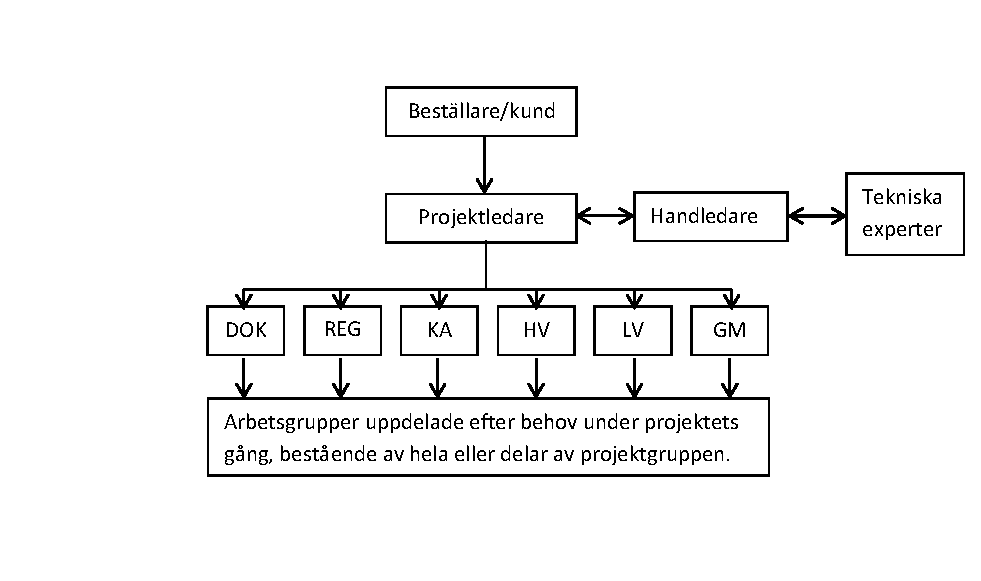
\includegraphics{organisation-figur.pdf}
	\caption{Översikt av ansvarsfördelning}
\end{figure}
Beställarens kontakt med gruppen sker huvudsakligen genom projektledaren. Varje gruppmedlem har ett eget ansvarsområde, och det ligger under projektledarens ansvar att se till att övriga gruppmedlemmar arbetar mot samma mål och att samtliga planerade aktiviteter har minst en huvudansvarig. Projektledaren ansvarar dessutom för att projektgruppen under projektets gång  delas in i mindre arbetsgrupper för att arbetsfördelningen inom gruppen, sett till nedlagda arbetstimmar,  skall bli så jämnt fördelad som möjligt.
Handledaren finns tillgänglig som vägledning för projektgruppen under hela projektets gång. Om gruppen har frågor rörande någon teknisk del av projektet kan handledaren hänvisa till en teknisk expert på området ifråga. Handledaren ska även godkänna vissa beslutspunkter för att projektet ska kunna fortskrida, se "Milstolpar och beslutspunkter".
\subsection{Villkor för samarbete inom projektgruppen}
\subsection{Definition av arbetsinnehåll och ansvar}


\section{Dokumentplan}	%%MJ
Test

\section{Utvecklingsmetodik}	%%SW

\section{ Utbildningplan}	%%Markus
\subsection{Egen utbildning}
Vid behov kommer medlemmarna i projektgruppen att kunna utbildas i de olika verktyg som ska användas under projektet. Exempel på sådana verktyg kan vara AVR Studio, C Programmering och alla de mätinstrument som kommer att vara nödvändiga. För att utbilda projektetgruppens medlemmar tillhandahåller kunden med Tekniska experter som kan ge korta lektioner. Innan Någon av de tekniska experterna anlitas kommer projektgruppen dock att tillfråga handledaren om inte denna kan hålla en kort intern utbildning.

\section{Rapporteringsplan}

\section{Mötesplan}

\section{Resursplan}	%%SW
\subsection{Personer}
\subsection{Materiel}
\subsection{Lokaler}
\subsection{Ekonomi}

\section{ Milstolpar och beslutspunkter} %%SL
Milstolpar för projektet bestäms inom gruppen, och sätts för att kunna kontrollera att tidsplanen följs som planerat. Varje milstolpe innefattar ett eller flera krav som ska vara uppfyllda och testade vid det datum som specifierats nedan. Beslutspunkter är krav uppsatta från beställaren. Vid varje beslutspunkt har beställaren rätt att besluta om projektet skall fortsätta eller ej.
\subsection{Milstolpar}

\begin{tabular}{|p{7mm}|p{117mm}|p{23mm}|}
        	\LIPSmilstolpe{\textbf{Nr}}{\textbf{Beskrivning}}{\textbf{Datum}}
	\LIPSmilstolpe{1}{Designspecifikationen accepterad av handledaren}{2012-03-16}
	\LIPSmilstolpe{2}{Bussen fungerar som den ska}{2012-03-30}
	\LIPSmilstolpe{3}{Data och mätvärden skickas via komunikationsenheten}{2012-04-05}
	\LIPSmilstolpe{4}{Roboten kan upptäcka korsningar}{2012-04-19}
	\LIPSmilstolpe{5}{Korrekt sensorinfo visas på PCn}{2012-04-20}
	\LIPSmilstolpe{6}{Motorn regleras autonomt utifrån sensorvärdena}{2012-04-27}
	\LIPSmilstolpe{7}{Styrkommandon utförs korrekt}{2012-05-04}
\hline
\end{tabular}

\subsection{Beslutspunkter}

\begin{tabular}{|p{7mm}|p{117mm}|p{23mm}|}
        	\LIPSmilstolpe{\textbf{BP}}{\textbf{Beskrivning}}{\textbf{Datum}}
	\LIPSmilstolpe{BP0}{Godkännande av projektdirektiv, beslut att starta förstudie}{2012-01-20}
	\LIPSmilstolpe{BP1}{Godkännande av kravspecifikation, beslut att starta förberedelsefasen}{2012-02-02}
	\LIPSmilstolpe{BP2}{Godkännande av projektplanering, beslut att starta utförandefasen}{2012-02-23}
	\LIPSmilstolpe{BP3}{Godkännande av designspecifikation, beslut att fortsätta utförandefasen}{2012-03-16}
	\LIPSmilstolpe{BP4}{Ej specifierad}{-}
	\LIPSmilstolpe{BP5}{Godkännande av produktens funktionalitet, beslut att leverera}{vecka 19}
	\LIPSmilstolpe{BP6}{Godkännande av leverans, beslut att upplösa projektgruppen}{2012-06-01}
\hline
\end{tabular}
\section{Aktiviteter}

\begin{tabular}{|p{7mm}|p{90mm}|p{23mm}|p{23mm}|}
	\LIPSleverans{\textbf{Nr}}{\textbf{Beskrivning}}{\textbf{Beroende av aktivitet nr}}{\textbf{Beräknad tid (h)}} 
	\LIPSaktivitet{Hoppa högt}{pi}{5 h}
\hline
\end{tabular}

\section{Tidplan}

\section{Förändringsplan}	%%Markus

\section{Kvalitetsplan}	%SL
För att säkerställa att kvaliten på roboten och dokumentationen används två medtoder, granskning och tester. Granskning rör all form av dokumentation som ingår i projektet. Dessutom kommer tester att göras kontinuerligt under projektet för att säkerställa att varje aktivitet ger önskat resultat.
\subsection{Granskningar}
Varje ny version av dokumentationen skall granskas av minst en gruppmedlem innan den anses färdig för inlämning. Om inget annat sägs är det dokumentansvarigs (Mattias Jansson) ansvar att dokumentet granskas. Syftet med granskningen är att kontrollera att dokumentet innehåller alla önskade delar och att det inte innehåller några grova språkliga eller utseendemässiga fel.
\subsection{Testplan}
Under projektet kommer tester utföras löpande för att säkerställa att arbetet ger önskat resultat. Gruppmedlemen som utsetts till testansvarig (Simon Wallin) är ansvarig för att planera och utföra testningen, samt att framställa en testplan som beskriver hur testerna ska genomföras och vilka krav som måste vara uppfyllda för att ett test ska godkännas.


\section{Riskanalys} %SW

\section{Prioriteringar}


\section{Projektavslut} %MARKUS


\newpage
\appendix
\section{Bilagor} \label{app:rules}


\subsection{Banspecifikation} \label{app:bana}

\newpage


\addcontentsline{toc}{section}{Referenser}
\begin{thebibliography}{99}
\bibitem{lipskompendiet}\textit{Projektmodellen LIPS - } Svensson, Tomas
\\Studentlitteratur, 2011.
\end{thebibliography}

\end{document} 

%%% Local Variables: 
%%% mode: latex
%%% TeX-master: t
%%% End: 
